\documentclass[a4paper]{article}
\usepackage[a4paper,top=1cm,bottom=2cm,left=2cm,right=2cm,marginparwidth=1.75cm]{geometry}
\usepackage{amsmath}
\usepackage{graphicx}
\usepackage[colorlinks=true, allcolors=blue]{hyperref}

\title{\textbf{EN2550 - Fundamentals of Image Processing and Machine Vision}\\
Assignment 02}
\author{Tharindu O.K.D.\\19062R}
\begin{document}
\maketitle
GitHub Repository : \url{https://github.com/dakshinatharindu/Image-Processing/blob/main/Assignment-02/190622R_a02.ipynb}

\section*{Question 01}
\begin{figure}[!htb]
    \centering
    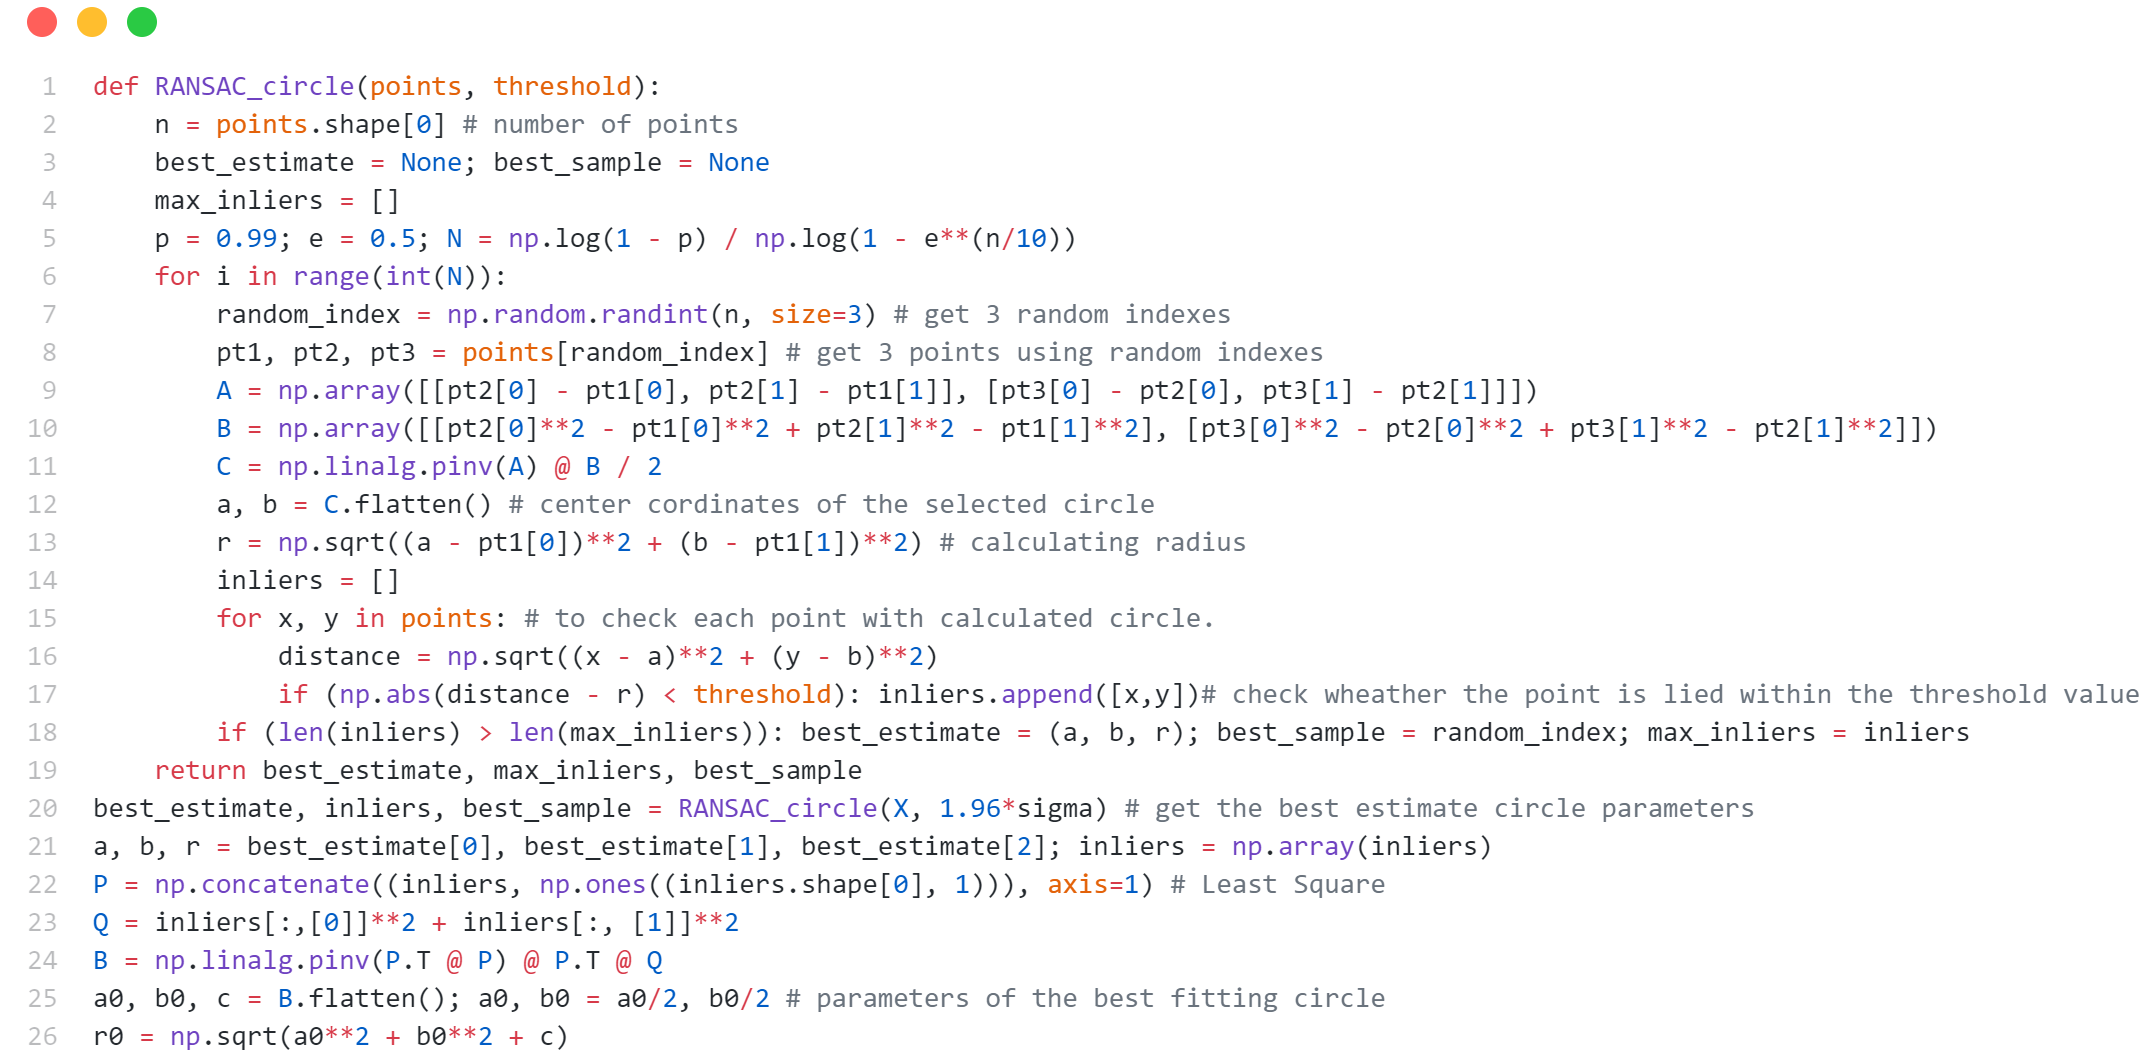
\includegraphics[width=\textwidth]{images/ransac_circle.png}
    \caption{$RANSAC\_circle$ function}
    \label{ransac_circle}
\end{figure}
Our objective of this function is to robustly fit a circle to our point set. This can be done using RANSAC
algorithm. Figure 1 shows the code snipped of the RANSAC function.
 
\subsubsection*{RANSAC Algorithm Explained}
\begin{enumerate}
  \item First, we calculate the number of iterations $N$ required to get a better estimation. We choose $N$ 
  so that, with probability $p$, at least one random sample is free from outliers.
  It is given by, $N=\frac{\log{(1-p)}}{\log{(1-(1-e)^n)}}$. Here $e$ is outlier
  ratio and $n$ is a number of points. Here I took $e=0.5$ and $p=0.99$ so 
  that 50\% of points will fall into inliers with a 99\% probability.
  \item We randomly select 3 points from the given data set. Then we calculate the fitting
   circle using these 3 points as follows.
   $$(x-a)^2+(y-b)^2=r^2$$substituting 3 point coordinates and putting it into matrix form, we get
   \begin{align*}
     \begin{pmatrix}
       x_2-x_1 & y_2-y_1\\
       x_3-x_2 & y_3-y_2
     \end{pmatrix}
     \begin{pmatrix}
       2a\\
       2b
     \end{pmatrix}&=
     \begin{pmatrix}
      x_2^2-x_1^2 & y_2^2-y_1^2\\
      x_3^2-x_2^2 & y_3^2-y_2^2
    \end{pmatrix}\\
    AC&=B\\
    C&=A^{-1}B
   \end{align*}
   Then we can find center coordinates and radius using the $C$ matrix.
   \item Then determine the inlier set 
   $$inliers=\{(x_i,y_i)\in points \text{ such that }|\sqrt{(x_i-a)^2+(y_i-b)^2}-r|<threshold\}$$
   \item If $|inliers|>|max\_inliers|$, we select it as the best estimate. Go to step 2
   until iterate N times.
  \end{enumerate}

  \subsubsection*{Finding Best Fitting Circle}

\begin{figure}[!htb]
  \centering
  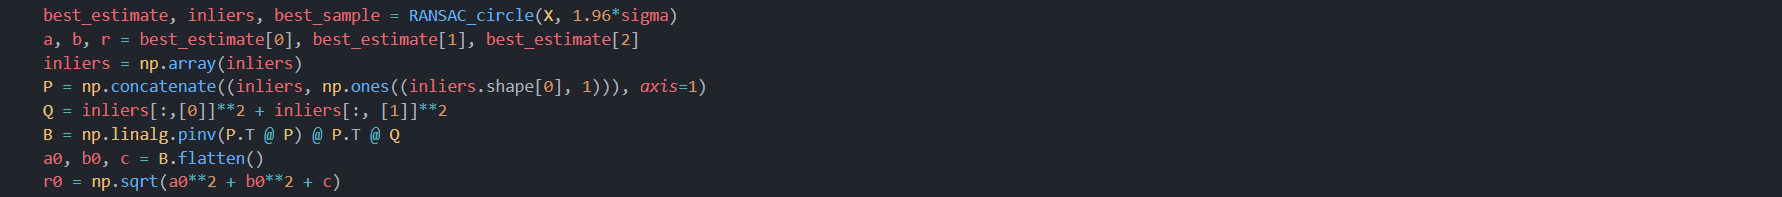
\includegraphics[width=\textwidth]{images/best_fit.png}
  \caption{Finding Best Fitting Circle}
  \label{bestfit}
\end{figure}
First, we get the parameters of the best fitting circle using the above 
$RANSAC\_circle$ function. Since the sample noise is distributed as zero-mean
 Gaussian, we pass the threshold value as $1.96\sigma$ so that will give
  a $\approx95\%$ probability of capturing all inliers. After
   finding the best inliers, we find the best fitting circle for
    those inliers using the Least Square approach as follows.
    \begin{align*}
      \begin{pmatrix}
        x_1 & y_1 & 1\\
        x_2 & y_2 & 1\\
        \vdots & \vdots & \vdots\\
        x_n & y_n & 1\\
      \end{pmatrix}
      \begin{pmatrix}
        2a_0 \\ 2b_0 \\ c
      \end{pmatrix}&=
      \begin{pmatrix}
        x_1^2 & y_1^2\\
        x_2^2 & y_2^2\\
        \vdots & \vdots \\
        x_n^2 & y_n^2\\
      \end{pmatrix}\\
      PB&=Q\\
      B&=(P^T P)^{-1}P^T Q
    \end{align*}
    Using the B matrix, we can find
     $a_0, b_0$, and $r_0$ which are the parameters of the best-fitting
      circle.
\begin{figure}[!htb]
  \centering
  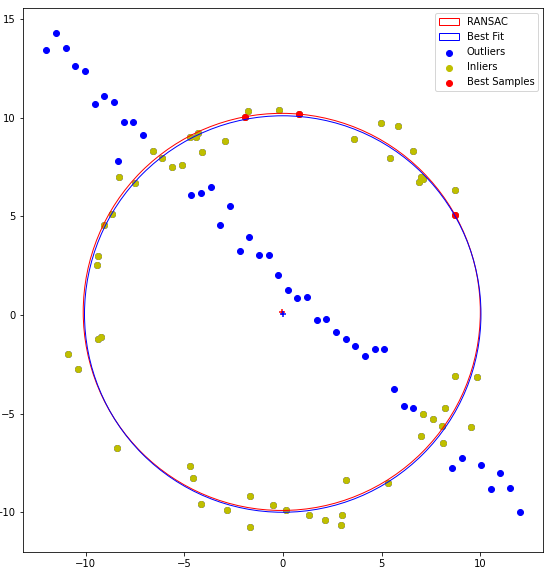
\includegraphics[width=0.5\textwidth]{images/ransac.png}
  \caption{Output}
  \label{ransac}
\end{figure}
\section*{Question 02}
\begin{figure}[!htb]
  \centering
  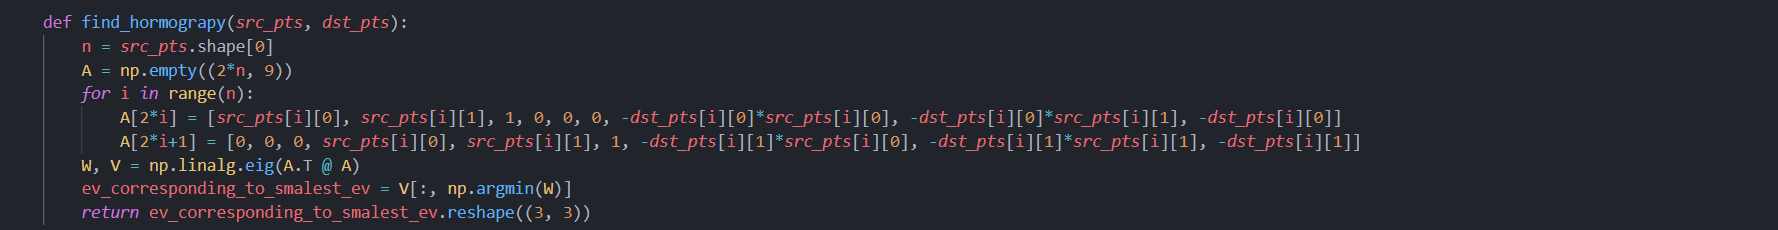
\includegraphics[width=\textwidth]{images/find_hormo.png}
  \caption{find\_hormography Code}
  \label{find_hormography}
\end{figure}

\begin{figure}[!htb]
  \centering
  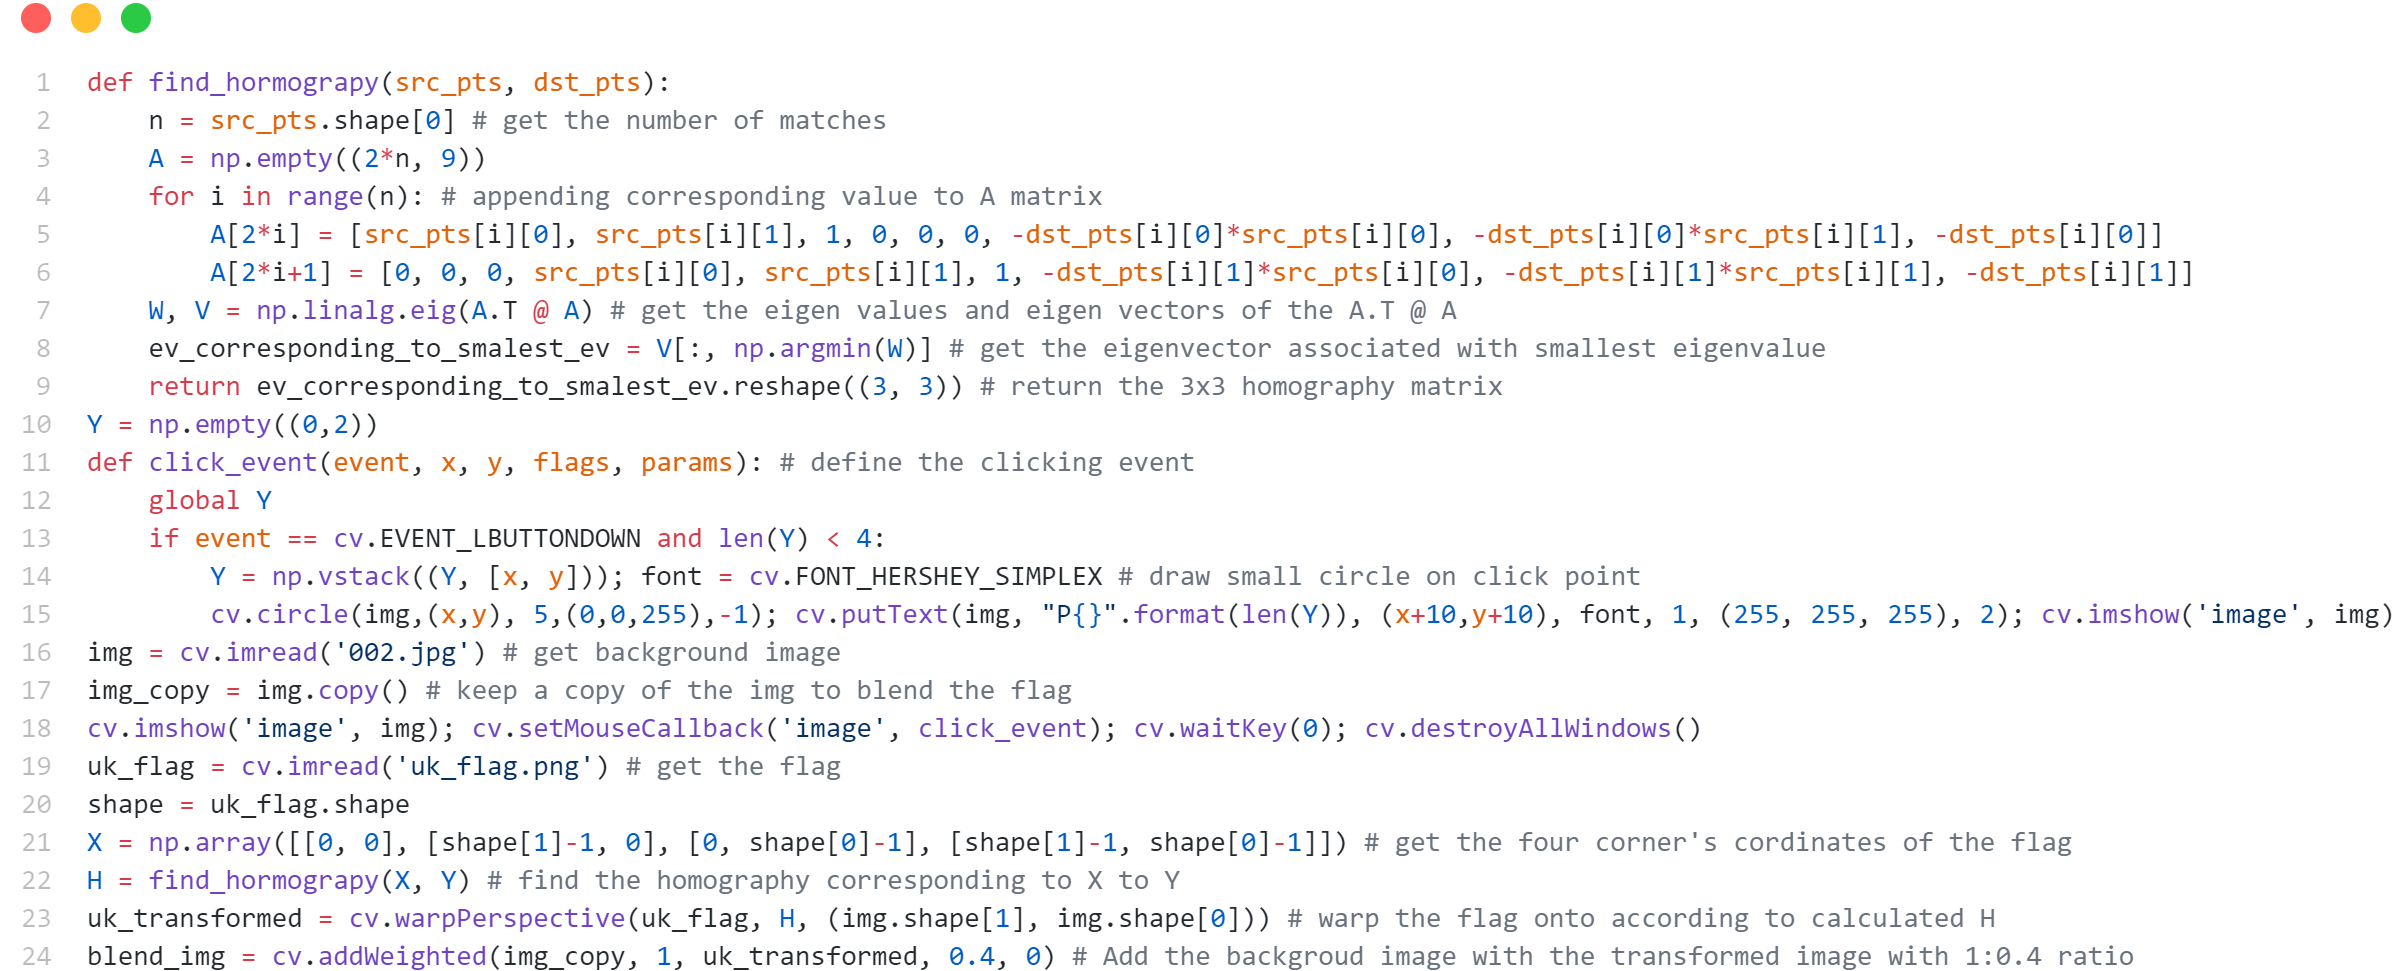
\includegraphics[width=\textwidth]{images/q2code.png}
  \caption{Code}
  \label{q2code}
\end{figure}

\begin{figure}[!htb]
  \centering
  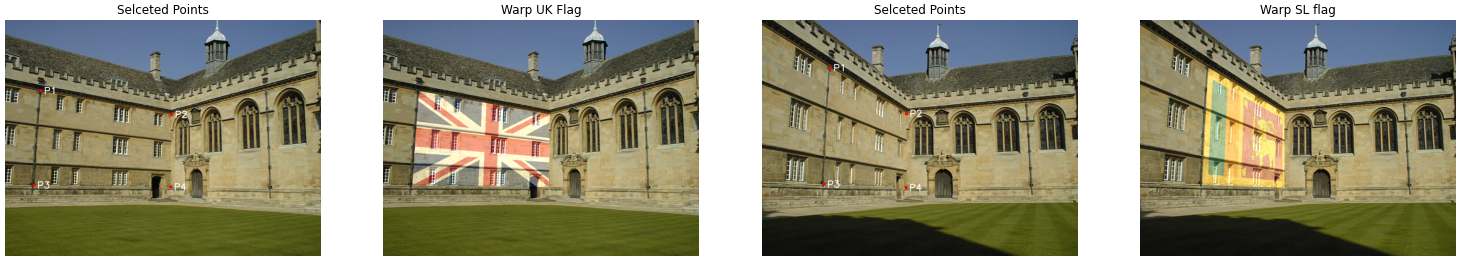
\includegraphics[width=\textwidth]{images/q22.png}
  \caption{Output}
  \label{q2}
\end{figure}
\end{document}
